\section{Entwicklung von UI-Tests}


Die Entwicklung von UI-Tests ist der zentrale Punkt dieser Arbeit. Im
Gegensatz zu Performance- und Sicherheitstests, die nicht funktional sind,
ist das Hauptziel dieser UI-Tests festzustellen, ob die beiden Versionen von
jExam so funktionieren, wie die Entwickler es beabsichtigt haben.
Dieses Kapitel konzentriert sich auf die Entwicklung der UI-Tests, die
verschiedenen Tools und die Design Patterns, die verwendet wurden. Zunächst
werden die verschiedenen Werkzeuge vorgestellt, die bei der Entwicklung
verwendet wurden. Anschließend werden die Design Patterns vorgestellt, die
dabei helfen, den Code robust und leicht wartbar zu machen. In Teil drei
wird der Schwerpunkt auf die Implementierung von Tests gelegt, und im letzten
Teil werden die erzielten Ergebnisse und zusätzliche Funktionen vorgestellt.

\subsection{Verwendete Werkzeuge}

\subsubsection{Selenium Webdriver}

Selenium ist ein Open-Source-projekt für eine Reihe von Tools und Bibliotheken
zur Unterstützung der Webbrowser-Automatisierung (vgl. \cite{selenium-survey}).
Selenium bietet  Werkzeuge zur Erstellung funktionaler Tests, ohne dass eine
Testskriptsprache erlernt werden muss. Außerdem bietet es eine testspezifische
Sprache (Selenese), mit der Tests in einer Reihe beliebter Programmiersprachen
geschrieben werden können, darunter JavaScript (Node.js), C#, Groovy, Java,
Perl, PHP, Python, Ruby und Scala. Die Tests können dann mit den meisten
modernen Webbrowsern ausgeführt werden. Selenium läuft auf Windows, Linux
und macOS. Selenium besteht aus mehreren Komponenten, von denen jede eine
bestimmte Rolle bei der Entwicklung der Testautomatisierung von Webanwendungen
übernimmt. Zu diesen Komponenten gehören: die Selenium IDE, Selenium Client API,
Selenium Remote Control, Selenium Grid und schließlich der Selenium WebDriver,
der in dieser Arbeit verwendet wird.

Das Kernelement von Selenium ist Selenium WebDriver, eine Schnittstelle zum
Schreiben von Anweisungen, die in verschiedenen Browsern austauschbar sind.
Selenium WebDriver nimmt Befehle entgegen (die in \gls{selenese} oder über eine
Client-API gesendet werden) und sendet sie an einen Browser. Dies wird durch
einen browserspezifischen Browsertreiber implementiert, der Befehle an einen
Browser sendet und Ergebnisse abruft. Die meisten Browsertreiber starten
tatsächlich eine Browseranwendung (z. B. Firefox, Google Chrome, Internet
Explorer, Safari oder Microsoft Edge) und greifen darauf zu. Selenium WebDriver
benötigt keinen speziellen Server, um Tests auszuführen. Stattdessen startet
der WebDriver direkt eine Browserinstanz und steuert sie.  Wo immer möglich,
verwendet WebDriver native Funktionen auf Betriebssystemebene und nicht
browserbasierte JavaScript-Befehle zur Steuerung des Browsers. Dadurch werden
Probleme mit subtilen Unterschieden zwischen nativen und JavaScript-Befehlen,
einschließlich Sicherheitseinschränkungen, vermieden (vgl. \cite{Stewart2016}).
Selenium WebDriver ist vollständig implementiert und wird in JavaScript
(Node.js), Python, Ruby, Java, Kotlin und C# unterstützt.


Selenium ist derzeit das von Testern am meisten geliebte Framework für
UI-Testing (vgl. \cite{selenium-survey} , S. 08-09). Es hat viele Vorteile,
wie z.B. die \"Ubertragbarkeit auf alle Systeme, die einfache Integration mit
andere Technologien, eine große und dynamische Entwicklergemeinschaft sowie
die Dokumentation und die Fülle an verfügbaren Ressourcen. Im Rahmen dieser
Arbeit wird der Selenium Web Driver mit der Programmiersprache Java verwendet.
\subsubsection{TestNG}

TestNG ist ein Open-Source-Testautomatisierungs-Framework für Java. Es wird
nach dem Vorbild von JUnit und NUnit entwickelt. Einige fortgeschrittene und
nützliche Funktionen, die TestNG bietet, machen es zu einem robusteren
Framework im Vergleich zu seinen Mitbewerbern (vgl. \cite{browserstack}).
Das NG in TestNG steht für "Next Generation". Es wird immer häufiger von
Entwicklern und Testern bei der Erstellung von Testfällen verwendet, da es
einfach ist, mehrere Annotationen, Gruppierungen, Abhängigkeiten,
Priorisierungen und Parametrierungsfunktionen zu verwenden. Durch die
Beseitigung der meisten Einschränkungen des älteren Frameworks gibt TestNG
dem Entwickler die Möglichkeit, flexiblere und leistungsfähigere Tests zu
schreiben.

Der Hauptgrund, warum TestNG für die Entwicklung der Tests in dieser
Arbeit ausgewählt wurde, ist in erster Linie die Tatsache, dass es im
Vergleich zu seinem Konkurrenten JUnit mehr nützliche Funktionen
bietet (vgl. \cite{browserstack}):

\begin{enumerate}
    \item Annotationen von TestNG sind im Vergleich zu JUnit
    einfacher zu verstehen
    \item TestNG erfordert im Gegensatz zu JUnit keine
    obligatorische Deklaration von @BeforeClass und @AfterClass
    \item Die Funktion der Parametrisierung, die TestNG bietet, ist
    bequemer und einfacher durch den Datenprovider zu nutzen.
    \item Funktionen wie Priorisierung und Gruppierung von Tests,
    die von TestNG bereitgestellt werden, machen es im Vergleich zu
    JUnit realistischer und leichter anpassbar.
    \item TestNG bietet im Vergleich zu JUnit in mehrfacher
    Hinsicht die Möglichkeit der parallelen Testausführung.

\end{enumerate}

Neben diesen Vorteilen gegenüber JUnit lässt sich TestNG leicht in das
Selenium-Framework integrieren. Dies macht es zu einem der am häufigsten
verwendeten Werkzeuge für das Schreiben von Selenium-Testskripten
(vgl. \cite{selenium-survey}, S.13).

\subsection{Entwurfsmuster}\label{subsec:entwurfsmuster}


Zu den Voraussetzungen, die von der Testinfrastruktur erwartet werden,
gehört die Hohe Wartbarkeit der Testsuite. Dieses Ziel könnte ohne die
Verwendung von Entwurfsmustern nicht erreicht werden. Entwurfsmuster
können den Entwicklungsprozess beschleunigen, indem sie getestete, bewährte
Entwicklungsparadigmen bereitstellen. Ein effektiver Softwareentwurf
erfordert die Berücksichtigung von Problemen, die möglicherweise erst
später bei der Implementierung sichtbar werden. Die Wiederverwendung von
Entwurfsmustern hilft, subtile Probleme zu vermeiden, die zu großen
Problemen führen können, und verbessert die Lesbarkeit des Codes für
Programmierer und Architekten, die mit den Mustern vertraut sind.  Für die
Entwicklung von Tests mit Selenium gibt es zwei Entwurfsmuster, die sehr
beliebt sind und von Testern verwendet werden :
\textbf{Page Object} und \textbf{Factory} (vgl. \cite{pattern-browser}).

\subsubsection{Page Object Model}

Page Object Model ist ein in Selenium verwendetes Entwurfsmuster,
bei dem ein Objektrepository zur Speicherung von WebElementen
erstellt wird. Es wird eine Java-Klasse erstellt, die jeder WebSeite
entspricht (siehe \Cref{fig:page-obj}). Diese Seiten bestehen aus WebElementen und den
entsprechenden Methoden, die auf diese Elemente einwirken (siehe \Cref{fig:page-exp}).
Alle Webseitenelemente befinden sich in einer Java-Klasse, indem sie durch
ihre Locators identifiziert werden.  Darüber hinaus werden für die
verschiedenen Seiten der Webseite mehrere Java-Klassen erstellt. Diese
Java-Klassen dienen als Repository, in dem die verschiedenen Elemente
gespeichert werden, mit denen Testfällen interagieren können. Die Verwendung
des Page Object Model hat viele Vorteile:

\begin{enumerate}
    \item \textbf{Erleichtert die Wartung des Codes} : Da die Testklassen von den
    Klassen getrennt sind, die die Webelemente und die Operationen auf
    ihnen enthalten, ist die Aktualisierung des Codes sehr einfach, wenn
    ein Webelement aktualisiert oder ein neues hinzugefügt wird.
    \item \textbf{Erleichtert die Lesbarkeit des Codes} : Der Benutzer kann das Projekt
    und die Testskripte aufgrund der feinen Trennung zwischen den Testklassen
    und den verschiedenen Webseiten leicht durchlesen.
    \item \textbf{Wiederverwendbarkeit des Codes} : Wenn mehrere Testskripte dieselben
    Webelemente verwenden, müssen nicht in jedem Testskript Code zur
    Behandlung des Webelements geschrieben werden. Die Unterbringung in einer
    separaten Seitenklasse macht es wiederverwendbar, indem es von jedem
    Testskript aus zugänglich gemacht wird.
\end{enumerate}

\begin{figure}[H]
    \centering
    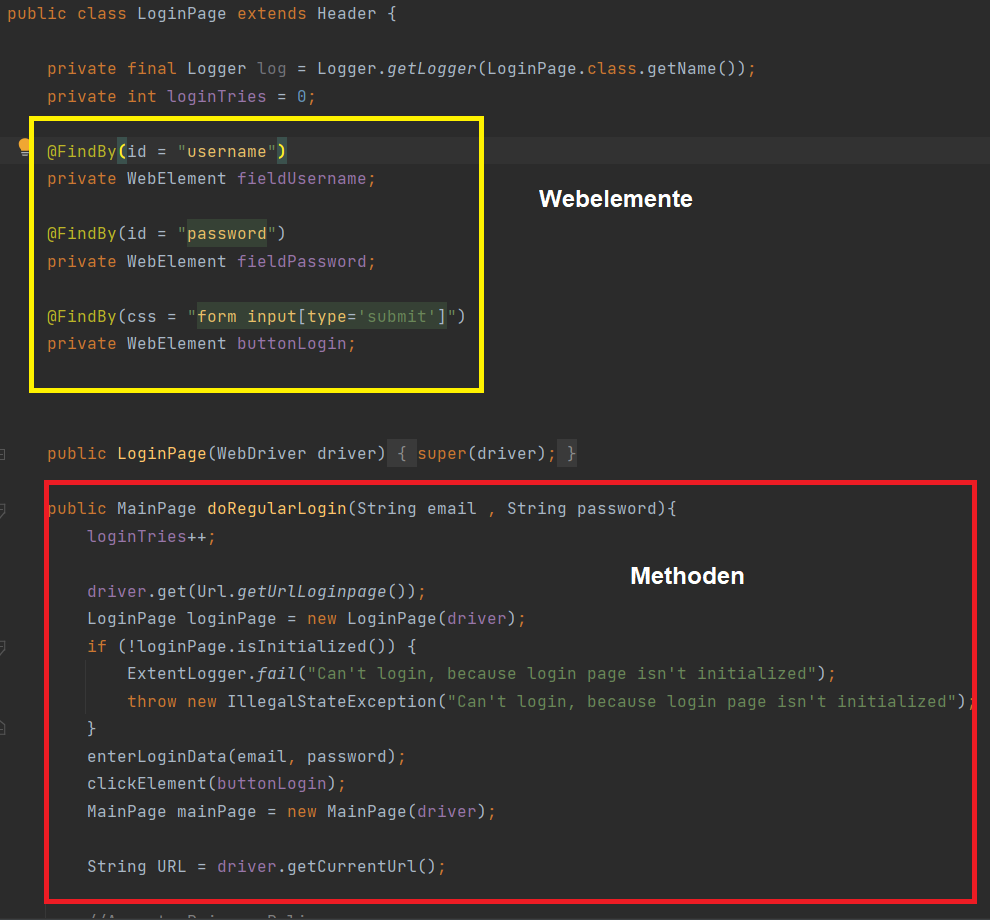
\includegraphics[scale=0.5]{images/page-example}
    \caption{Darstellung der jExam LoginPage mit dem Page Object Model} \label{fig:page-exp}
\end{figure}

\begin{figure}[H]
    \centering
    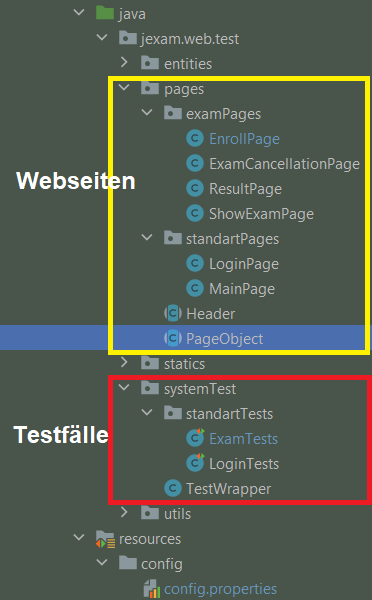
\includegraphics[scale=0.6]{images/page-object}
    \caption{Projektstruktur von jExam Page Object Model} \label{fig:page-obj}
\end{figure}

\subsubsection{Factory}

Page Factory ist eine Klasse, die von Selenium WebDriver bereitgestellt
wird, um das Page Object Model zu implementieren. Das Page Object
Repository wird mit Hilfe des Page Factory-Konzepts von den Testmethoden
getrennt. Page Factory bietet Annotationen, um Elemente zu initialisieren und sie
anschaulich und lesbar macht. Zu den Vorteilen seiner Verwendung gehören:

\begin{enumerate}
    \item \textbf{Sauberer Code}: Das definierte Webelement wird von den Methoden
    getrennt, um eine Webseite in einer Page Object sauber und
    aufgeräumt zu gestalten.
    \item \textbf{Lesbar und beschreibend}: Ein Webelement wird als Variable
    (bekannt als Object Field) deklariert, und die Field-Annotation
    (@FindBy siehe \Cref{fig:page-exp}) wird verwendet, um den Namen, den Typ und
    die Position des Elements zu beschreiben. Auf diese Weise können
    definierte Webelement anhand seiner Annotationen wie Name, Typ
    usw. leicht identifiziert werden.
    \item \textbf{Einfache Wartbarkeit}: Das definierte Webelement kann ohne
    Neudefinition überall in der Page Object Klasse und den Unterklassen
    verwendet werden. Das bedeutet, dass ein bestimmtes Webelement
    mehrmals verwendet werden kann, aber nur an einer Stelle
    definiert ist.
\end{enumerate}


Im nächsten Teil werden die Implementierung der Tests und die verwendeten
Methoden genauer beschrieben.





\subsection{Implementierung der Testsuite}

Das Schreiben eines UI-Tests mit Selenium ist ein Prozess, der je
nach der zu testenden Funktionalität mehr oder weniger lange dauert.
Je komplexer die Funktionalität ist, desto komplexer ist auch das
Schreiben des Tests. In diesem Kapitel geht es darum, den Prozess
der Testimplementierung zu beschreiben. Dazu wird ein Test verwendet,
der als Beispiel für die Beschreibung des Implementierungsprozesses
dienen soll : \textbf{Der Registrierungstest}. Dieser Test wurde ausgewählt,
weil er fast alle Funktionen abdeckt, die bei der Erstellung der
anderen Tests verwendet wurden. Das Schreiben von Tests ist in fünf
Phasen unterteilt:

\subsubsection{Phase 1: Initialisierung der Daten}

Vor der Durchführung von Tests ist es wichtig, die zu testende
Plattform mit Daten vorzubereiten. Dies ermöglicht es, die
Ausgangssituation der Plattform, die man testen möchte, zu
reproduzieren. Wenn beispielsweise die Verbindung eines Benutzers
mit einer Plattform getestet werden soll, ist es wichtig, dass die
Daten dieses Benutzers bereits in der Datenbank vorhanden sind.

Im aktuellen Fall wird dies von einem Docker-Container namens
Initializer (wird im Kapitel über Docker ausführlich behandelt)
durchgeführt, dessen Zweck  ist, ein Skript auszuführen, das Daten
in den JBoss-Server von jExam einspeist. Im Falle des
Registrierungstests wird eine gültige, aber nicht auf der
Plattform registrierte Matrikelnummer generiert (siehe \Cref{fig:testData}).

\begin{figure}[H]
    \centering
    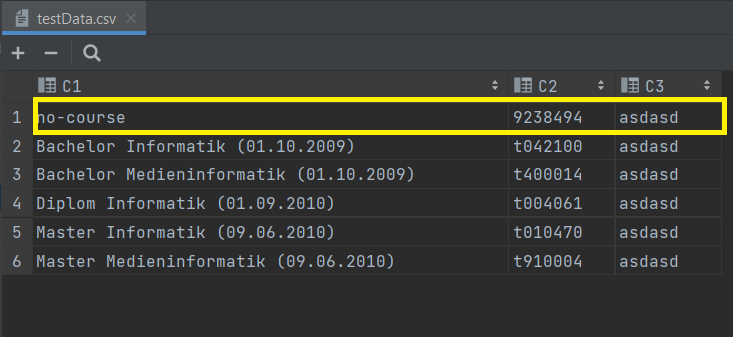
\includegraphics[scale=0.7]{images/testData}
    \caption{Vom Initializer erzeugte CSV-Daten} \label{fig:testData}
\end{figure}
\subsubsection{Phase 2: Erstellung eines Testszenarios}

In dieser Phase muss der Tester ein Ausführungsszenario für seinen 
Test erstellen. Es geht darum, die zu testende Funktion manuell
auf der Plattform auszuführen und die Ausführungsschritte zu 
dokumentieren, die in den nächsten Schritten automatisch wiederholt
werden. Dieser Prozess könnte auch in schriftlicher Form erfolgen
(normalerweise bei langen Szenarien). Diese Phase dient dazu, den 
Test im Detail zu planen und so die spätere Umsetzung zu erleichtern.
Im Falle des Registrierungstests ist das Szenario wie folgt festgelegt:

\begin{enumerate}
    \item Gehen Sie auf die Login-Seite und füllen Sie das Formular mit
    der nicht registrierten Matrikelnummer aus.
    \item Klicken Sie auf den Login-Button und Sie werden zur
    Registrierungsseite weitergeleitet.
    \item Füllen Sie das Registrierungsformular aus und klicken Sie
    auf Registrieren.
    \item Weiterleitung zur Seite Privacy Policy und Zustimmung zu
    den allgemeinen Nutzungsbedingungen
    (prüfen Sie, ob der TestUser automatisch eingeloggt wird).
    \item Logout und Login erneut mit den Zugangsdaten und der
    Matrikelnummer, die Sie bei der Registrierung verwendet haben.
    \item Wenn alles richtig funktioniert: Die Registrierung war erfolgreich.
\end{enumerate}
\subsubsection{Phase 3: Erstellung von Objekt-Seiten}

Wie bereits im \autoref{subsec:entwurfsmuster} erwähnt, wird das Object
Page Entwurfsmuster für die Erstellung von Tests verwendet.
Vor der Implementierung des Szenarios muss der Tester zunächst
die Objekte und Seiten erstellen, die für die Ausführung des Szenarios
erforderlich sind. Im Rahmen des Registrierungstests müssen folgende
Seiten erstellt werden: LoginPage, RegistrationPage, ContractPage
(Privacy Policy) und die MainPage. Wenn die RegistrationPage
im Detail betrachtet wird, kann man feststellen, dass diese
Java-Klasse (wie alle anderen Object-Seiten) einige besondere Merkmale
aufweist.

Zunächst erbt sie von der Klasse Header (die den auf allen Seiten
vorhandenen Header repräsentiert). Der Header selbst stammt von
PageObject ab, das die Grundstruktur einer Seite repräsentiert
(siehe \Cref{fig:pag-uml}). Die Klassen Header und PageObject enthalten
Webelelemente und Methoden, die normalerweise auf allen Seiten der
Anwendung zugänglich sind. Dadurch kann das Design Pattern Page
Object optimal genutzt werden.

\begin{figure}[H]
    \centering
    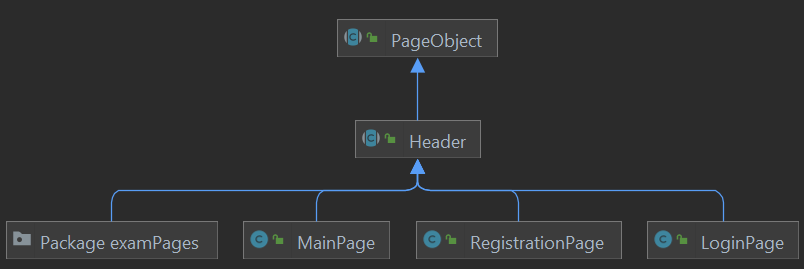
\includegraphics[scale=0.7]{images/pag-uml}
    \caption{UML Diagramm für die Java Page-Objekte} \label{fig:pag-uml}
\end{figure}

Zweitens enthält die Registrationpage eigene Webelemente.
Zum Beispiel die verschiedenen Inputs des auszufüllenden Formulare und
die anzuklickenden Bestätigungsbuttons (siehe Quellcode \ref{lst:registerpage}). Darüber hinaus
verfügt die Seite über die Methode registerUser, die ein
Formularobjekt (RegistrationForm) als Parameter hat und alle Eingaben
des Formulars ausfüllt und die ContractPage zurückgibt.

\begin{lstlisting}[label={lst:registerpage}, caption={RegistrationPage Quellcode}]
// RegistrationPage.java

    public class RegistrationPage extends Header {

    @FindBy(id = "cfirstname")
    private WebElement fieldFirstName;

    @FindBy(id = "csurname")
    private WebElement fieldName;

    @FindBy(id = "cmatrikel")
    private WebElement matrikel;

    public RegistrationPage(WebDriver driver) {
        super(driver);
    }

    @Override
    public boolean isInitialized() {
        WebElement h1_title;
        try{
            h1_title = driver.findElement(By.xpath("//H1[text()='Registrierung']"));
        }catch (NoSuchElementException e ){
            ExtentLogger.info("Main Title was not found");
            return false;
        }
        return h1_title.isDisplayed();
    }


    public ContractPage registerUser(RegistrationForm registrationForm){

        sendKeysToElement(fieldFirstName, registrationForm.firstName);
        sendKeysToElement(fieldName, registrationForm.lastName);

        Select fieldGender = new Select(driver.findElement(By.id("cgender")));
        fieldGender.selectByValue(registrationForm.gender);

        Select fieldCountry = new Select(driver.findElement(By.id("ccountry")));
        fieldCountry.selectByValue(registrationForm.country);

        Select fieldLanguage = new Select(driver.findElement(By.id("clanguage")));
        fieldLanguage.selectByValue(registrationForm.defaultLanguage);


        matrikel.clear();
        sendKeysToElement(matrikel, registrationForm.matrikel);

        Select fieldFaculty = new Select(driver.findElement(By.id("ou-combo")));
        fieldFaculty.selectByValue(registrationForm.faculty);

        Select fieldDegree = new Select(driver.findElement(By.id("degree-combo")));
        fieldDegree.selectByValue(registrationForm.degree);

        Select fieldExamReg = new Select(driver.findElement(By.id("er-combo")));
        fieldExamReg.selectByValue(registrationForm.examRegulation);

        WebElement addFaculty = driver.findElement(By.id("addEr"));

        clickElement(addFaculty);

        WebElement validationBtn = driver.findElement(By.xpath("(//INPUT[@class='btn fill-primary'])[2]"));
        clickElement(validationBtn);

        return new ContractPage(driver);
    }
}
\end{lstlisting}
\subsubsection{Phase 4: Erstellen von Verbindungen zwischen den Seiten}

Wenn auf einen Link geklickt oder einfach ein Formular bestätigt wird,
wird man normalerweise auf eine andere Seite weitergeleitet. Diese Phase
befasst sich im Wesentlichen mit der Umsetzung dieser Aufgabe.
Im Rahmen der Implementierung des Registrierungstests geht es darum,
die Seiten zwischen zwei Aktionen miteinander zu verbinden.
Zum Beispiel sollte die Registrierungsfunktion nach einem Klick
auf den Button Login die RegisterPage zurückgeben (siehe \Cref{fig:reg-page}).
Dies ist in der Tat eine Modellierung der Web-Navigation in Java.
Diese Arbeit muss durchgeführt werden und macht in der letzten Phase
Sinn.

\begin{figure}[H]
    \centering
    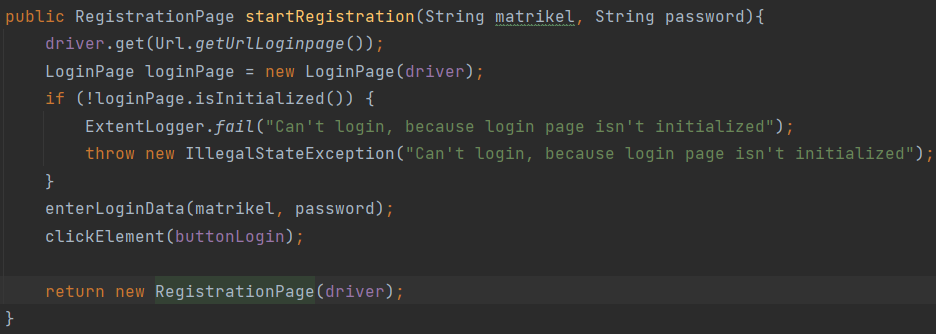
\includegraphics[scale=0.5]{images/reg-page}
    \caption{StartRegistration Funktion} \label{fig:reg-page}
\end{figure}

\subsubsection{Phase 5: Implementierung der tests nach dem szenario}

Diese Phase konzentriert sich auf die Umsetzung des in Phase 2
beschriebenen Szenarios. Es handelt sich um das Schreiben des Tests
an sich. In dieser Phase wird der Tester die Aktionen eines Nutzers
nacheinander ausführen.

Im Fall des Registrierungstests geht es zunächst darum, sich mit einer
Matrikelnummer zu registrieren, die nicht in der Datenbank verzeichnet
ist. Dann wird das Registrierungsformular mit den zuvor festgelegten
Daten ausgefüllt. Im nächsten Schritt werden die Allgemeinen
Geschäftsbedingungen akzeptiert und der Testuser dann einloggt.
Um zu überprüfen, ob die Registrierung erfolgreich war, muss der
Tester einen Login-Test mit den Daten simulieren, die er bei der
Registrierung verwendet hat (siehe Quellcode \ref{lst:reg-test}). Zwischen all
diesen Schritten werden Verifikationsprozesse durchgeführt
(z. B. ob eine Seite korrekt initialisiert wurde).

Es ist wichtig, Logs und ExtentLogger zu verwenden, um jeden Schritt
der Tests zu dokumentieren. Dadurch kann bei der Erstellung des
Ausführungsberichts nachvollzogen werden, welche Schritte während
des Tests durchgeführt wurden. Außerdem können diese Logs zeigen,
ob die Tests abgeschlossen wurden oder ob während der Ausführung
ein Fehler aufgetreten ist.


\begin{lstlisting}[label={lst:reg-test}, caption={Registration Test Quellcode}]

    // Registration Test Quellcode

    @Test
    @Description("New User Registration")
    public void doRegistrationTest(){
        ExtentReport.createTest("Test User Registration");
        ExtentLogger.info("⛔⛔ If you dont see \"Test Passed\" at the end, the Test didn't passed !");

        TestUser user = TestUser.REGISTRATION_USER;
        RegistrationPage registrationPage = startRegistration(user.username, user.password);
        Assert.assertTrue(registrationPage.isInitialized(),"Registrationpage was not correctly initialized");
        ExtentLogger.info("Registration Page is correctly initialized !");

        RegistrationForm form = new RegistrationForm(user.username+"@", user.username+"@", "f",
                "DE", user.username, "30010", "Bachelor Informatik", "1533186");
        ContractPage contractPage = registrationPage.registerUser(form);
        Assert.assertTrue(contractPage.isInitialized(), "Contractpage should be initialized !");
        ExtentLogger.info("Contract Page is initialized");

        MainPage mainPage = contractPage.acceptPrivacyPolicy();
        ExtentLogger.info("Privacy Policy was accepted");

        ExtentLogger.info("Try logout and login !");
        LoginPage loginPage = mainPage.selectLogoutLink();
        Assert.assertTrue(loginPage.isInitialized() , "Expected to land on login page, after log in, but landed on another page");
        ExtentLogger.info("Logout was successful, got on login page");
        log.info("Logout was successful, got on login page");

        // New Login with New Identifier
        mainPage = regularLogin(user.username , user.password);
        Assert.assertTrue(mainPage.isInitialized() , "Expected to land on main page, after log in, but landed on another page");
        ExtentLogger.info("Login was successful, got on main page");
        log.info("Login was successful, got on main page");

        loginPage = mainPage.selectLogoutLink();
        Assert.assertTrue(loginPage.isInitialized() , "Expected to land on login page, after log in, but landed on another page");
        ExtentLogger.info("Logout was successful, got on login page");
        log.info("Logout was successful, got on login page");

        ExtentLogger.info("Registration was successful");
        log.info("Registration was successful");
        ExtentLogger.pass("Test passed");
    }
\end{lstlisting}

Es gibt noch viele weitere Funktionen und Klassen, die in dieser
Arbeit nicht beschrieben werden können. Die Details des Schreibens
und aller Funktionen werden jedoch in der Dokumentation der
Testinfrastruktur ausführlich erläutert.

\subsection{Erreichte Ergebnisse}
